% !TEX encoding = UTF-8 Unicode
\documentclass[
11pt,
master, % тип документа
subf, % подключить и настроить пакет subfig для вложенной нумерации рисунков
href, % подключить и настроить пакет hyperref
colorlinks=true, % цветные гиперссылки
times, % шрифт Times как основной
%fixint=false % отключить прямые знаки интегралов
]{disser}
\usepackage[left=25mm, top=20mm, right=10mm, bottom=20mm]{geometry}
\usepackage[T2A]{fontenc}
\usepackage[utf8]{inputenc}
\usepackage[english,russian]{babel}
\usepackage{amsmath,amssymb,cmap} % cmap для кодировки шрифтов в pdf
\usepackage{pdfpages} % вставляем pdf файлы
\usepackage{indentfirst} % отделять первую строку раздела абзацным отступом
\usepackage{titletoc} % убираем отступ перед "Оглавление"
\usepackage{graphicx}
\usepackage{setspace}
\usepackage{verbatim} % для оформления кода
\usepackage{pdfsync} % установка соответствия документ - код
\graphicspath{{./Img/}}

\setlength\parindent{5ex} % абзацный отступ равный пяти строчным буквам основного шрифта
\pagestyle{plain} % включаем нумерацию
\setcounter{tocdepth}{2} % включать подсекции в оглавление
\linespread{1.3} % полуторный интервал


% Номера страниц снизу и по центру
\pagestyle{footcenter}
\chapterpagestyle{footcenter}

\begin{document}
	
\pagestyle{empty}
\begin{center}
	
	\noindent  Федеральное государственное бюджетное образовательное учреждение\\
	высшего профессионального образования\\
	
	Московский государственный технический университет им. Н.Э. Баумана \\
	Факультет <<Фундаментальные науки>>\bigskip\\
	
	\vfill
	
	Домашнее задание\\
	по курсу «Вычислительная физика»\\
	на тему: «Решение жёстких систем дифференциальных уравнений»\\
	
	
	\vfill
	\vfill
	\begin{flushright}
		\begin{tabular}{ll}
			Выполнили: & студенты группы ФН4-72Б     \\
			& Хижик А.И., Мистрюкова Л.А.,  \\
			Проверил:  & доцент, к.физ.-мат.н.       \\
			& Хасаншин Р.Х.
		\end{tabular}
	\end{flushright}
	\vfill
	\begin{center}
		Москва, $2019$
	\end{center}
	
\end{center}
\pagebreak


\pagestyle{plain}
\tableofcontents

\section{Постановка задачи}
\begin{itemize}
  \item Решить дифференциальное уравнение $y' = -\lambda y$, $y(0) = 1$, $x \in [0,1]$ при $\lambda = 10^i$, $i = \overline{0,2}$, используя чисто неявную разностную схему четвёртого порядка
      $$u_{n+4} = \frac{48}{25}u_{n+3} - \frac{36}{25}u_{n+2} + \frac{16}{25}u_{n+1} + \frac{12}{25}hf(x_{n+4},u_{n+4}).$$
\end{itemize}

\newpage
\section{Результаты}

\subsection{$N=100$}

\begin{figure}[h!]
  \centering
  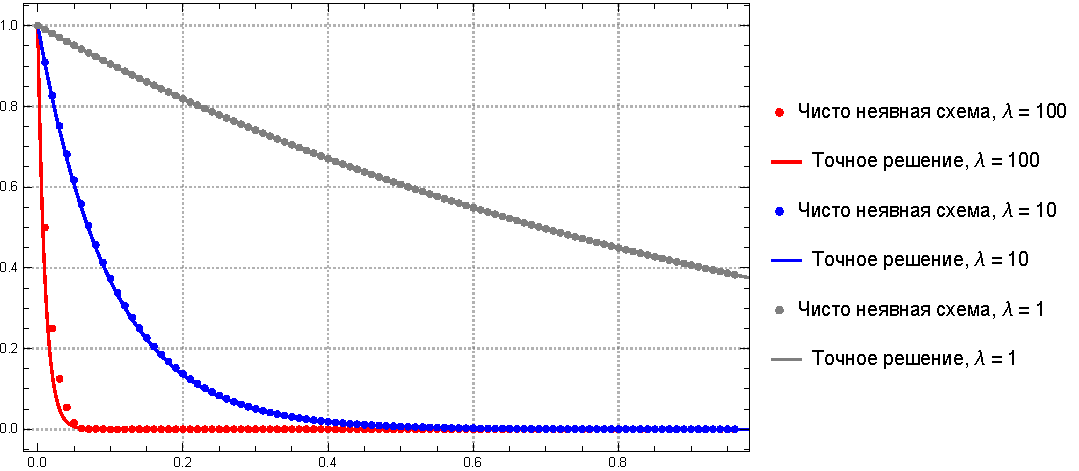
\includegraphics[width=0.8\linewidth]{pl1001}
  \caption{}\label{ris:1}
\end{figure}

\begin{figure}[h!]
  \centering
  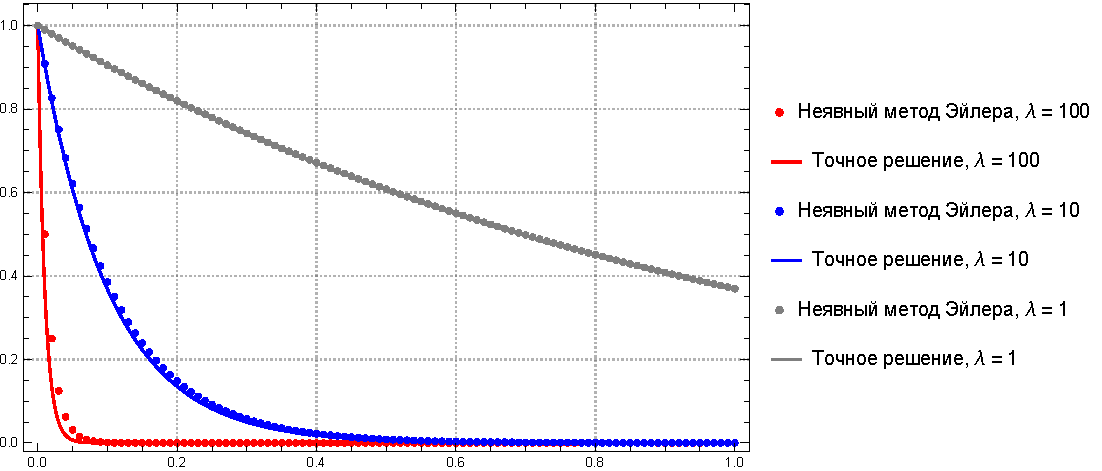
\includegraphics[width=0.8\linewidth]{pl1002}
  \caption{}\label{ris:2}
\end{figure}

\begin{figure}[h!]
  \centering
  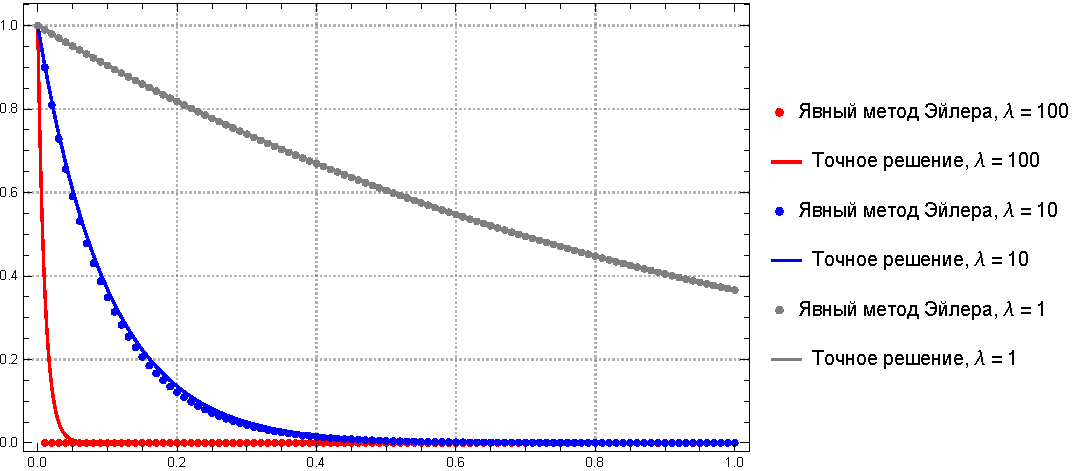
\includegraphics[width=0.8\linewidth]{pl1003}
  \caption{}\label{ris:3}
\end{figure}

\newpage
\subsection{$N=50$}

\begin{figure}[h!]
  \centering
  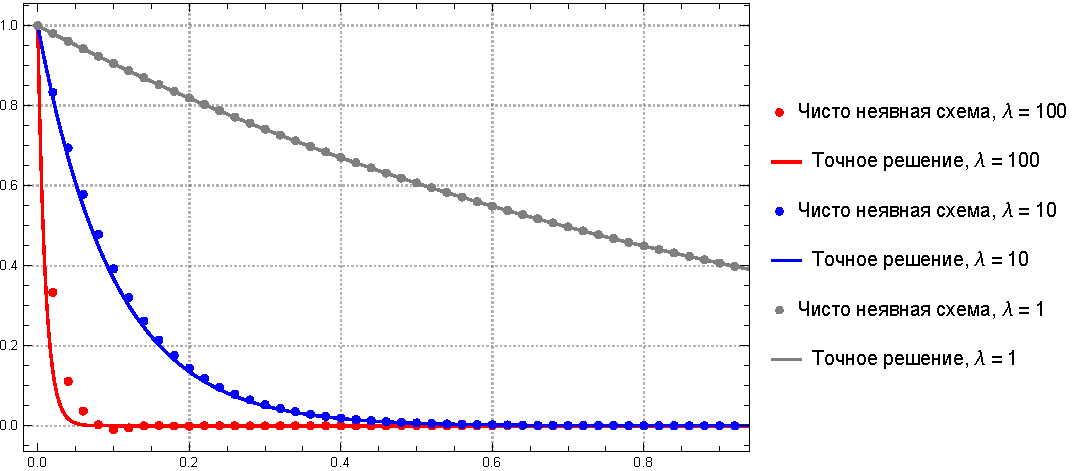
\includegraphics[width=0.8\linewidth]{pl501}
  \caption{}\label{ris:4}
\end{figure}

\begin{figure}[h!]
  \centering
  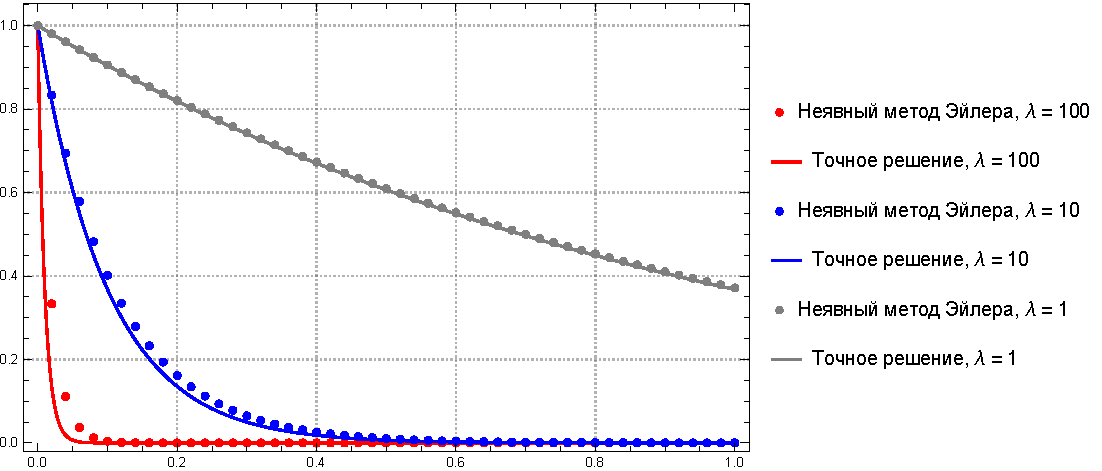
\includegraphics[width=0.8\linewidth]{pl502}
  \caption{}\label{ris:5}
\end{figure}

\begin{figure}[h!]
  \centering
  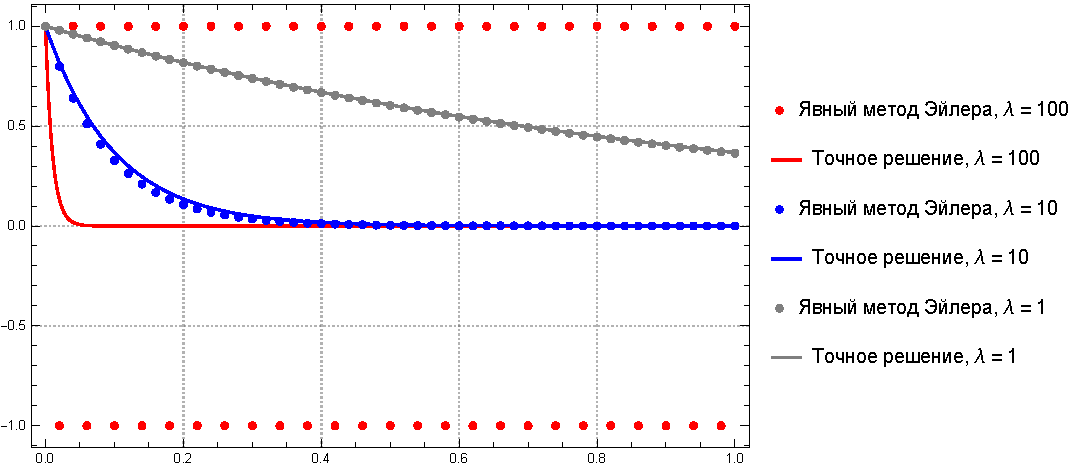
\includegraphics[width=0.8\linewidth]{pl503}
  \caption{}\label{ris:6}
\end{figure}

\subsection{$N=25$}

\begin{figure}[h!]
  \centering
  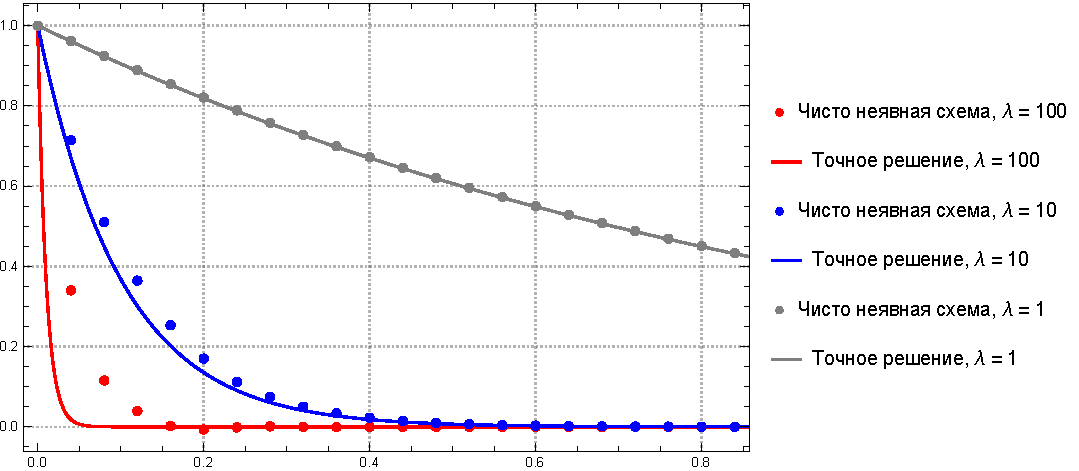
\includegraphics[width=0.8\linewidth]{pl251}
  \caption{}\label{ris:7}
\end{figure}

\begin{figure}[h!]
  \centering
  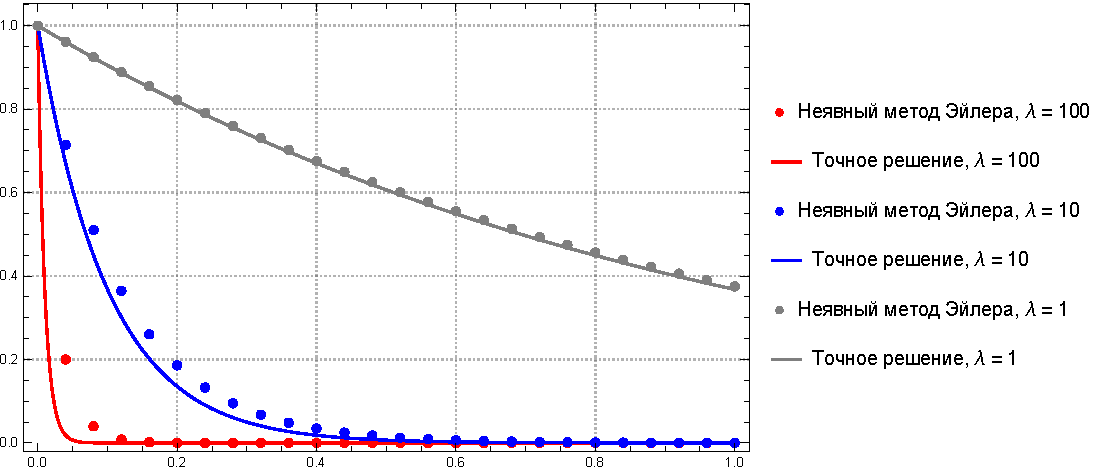
\includegraphics[width=0.8\linewidth]{pl253}
  \caption{}\label{ris:8}
\end{figure}

\begin{figure}[h!]
  \centering
  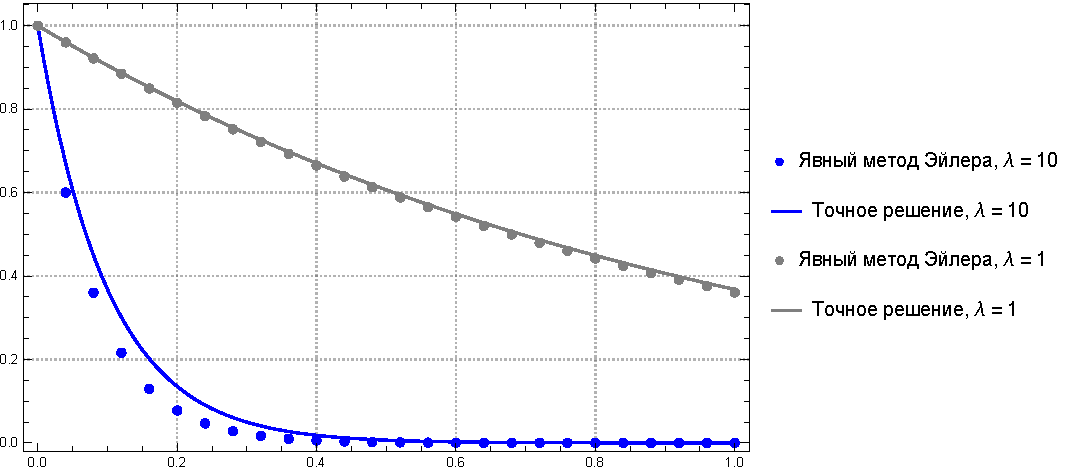
\includegraphics[width=0.8\linewidth]{pl252}
  \caption{}\label{ris:9}
\end{figure}

\newpage
\begin{figure}[h!]
  \centering
  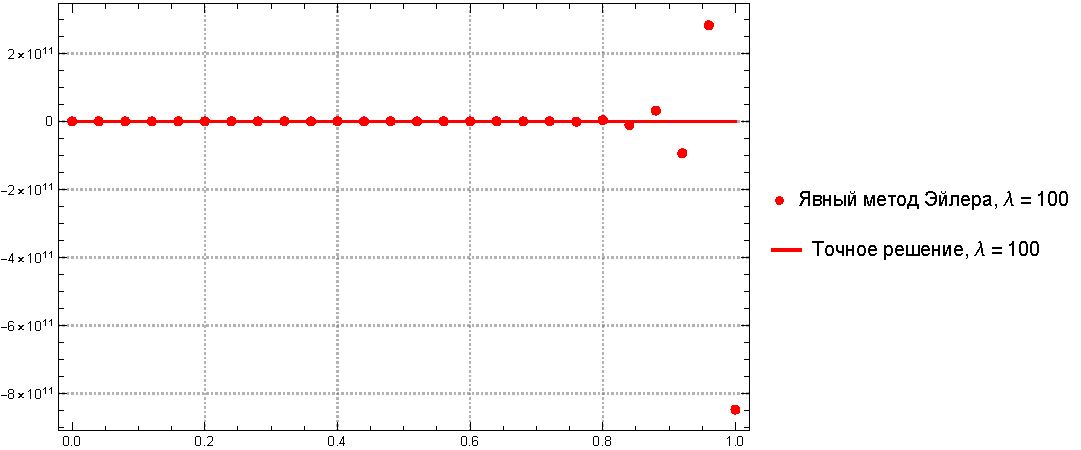
\includegraphics[width=0.8\linewidth]{pl2521}
  \caption{}\label{ris:10}
\end{figure}

\section{Вывод}
Решено дифференциальное уравнение $y' = -\lambda y$, $y(0) = 1$, $x \in [0,1]$ при $\lambda = 10^i$, $i = \overline{0,2}$, используя чисто неявную разностную схему четвёртого порядка $\displaystyle u_{n+4} = \frac{48}{25}u_{n+3} - \frac{36}{25}u_{n+2} + \frac{16}{25}u_{n+1}+\\ + \frac{12}{25}hf(x_{n+4},u_{n+4})$, явный и неявный методы Эйлера.

Наибольшую точность показала чисто неявная разностная схема четвёртого порядка. При нарушении условия устойчивости для явного методы Эйлера произошёл ``взрыв погрешности''.
\end{document} 